\documentclass[../../main/main.tex]{subfiles}
\graphicspath{{./figures/}}

\dominitoc
\faketableofcontents

% \renewcommand{\mtcSfont}{\small\bfseries}
% \renewcommand{\mtcSSfont}{\footnotesize}
\mtcsettitle{minitoc}{}
\mtcsetrules{*}{off}

\makeatletter
\renewcommand{\@chapapp}{Mécanique -- chapitre}
\renewcommand{\chaplett}{M}
\makeatother

% \toggletrue{student}
% \toggletrue{corrige}
% \renewcommand{\mycol}{black}
% \renewcommand{\mycol}{gray}

\hfuzz=5.002pt

\begin{document}
\setcounter{chapter}{0}

\settype{book}
\settype{prof}
\settype{stud}

\chapter{Cinématique du point en cartésiennes}

\vspace*{\fill}

\begin{tcn}(appl)<ctc>"somm"'t'{Sommaire}
	\let\item\olditem
	\vspace{-15pt}
	\minitoc
	\vspace{-25pt}
\end{tcn}

\begin{tcn}[sidebyside]
	(appl)<ctb>"how"'t'{Capacités exigibles}
	\begin{itemize}[label=\rcheck]
		\item Espace et temps classiques. Notion de référentiel. Caractère relatif
		      du mouvement. Caractère absolu des distances et des intervalles de
		      temps.
		\item Citer une situation où la description classique de l'espace ou du
		      temps est prise en défaut.

		\item Identifier les degrés de liberté d'un mouvement. Choisir un système
		      de coordonnées adapté au problème.

		\item Coordonnées cartésiennes~: exprimer à partir d'un schéma le
		      déplacement élémentaire, construire le trièdre local associé et en
		      déduire géométriquement les composantes du vecteur vitesse.
	\end{itemize}
	\tcblower
	\begin{itemize}[label=\rcheck]
		\item Établir les expressions des composantes des vecteurs position,
		      déplacement élémentaire, vitesse et accélération en coordonnées
		      cartésiennes.

		\item Mouvement à vecteur accélération constant~: exprimer le vecteur
		      vitesse et le vecteur position en fonction du temps. Établir
		      l'expression de la trajectoire en coordonnées cartésiennes.

		\item Situer qualitativement la direction du vecteur vitesse et du
		      vecteur accélération pour une trajectoire plane.
	\end{itemize}
\end{tcn}

\vspace*{\fill}
\newpage
\vspace*{\fill}

%\vspace{-15pt}
\begin{tcn}[%
		sidebyside, fontupper=\small, fontlower=\small
	](appl)<ctb>"chek"'t'{L'essentiel}
	\tce{defi}
	% \tce{rapp}
	\tce{prop}
	% \tce{theo}
	% \tce{loi}
	% \tce{coro}
	\tce{demo}
	% \tce{inte}
	% \tce{impl}
	% \tce{tool}
	% \tce{nota}
	% \tce{appl}
	% \tce{rema}
	% \tce{exem}
	% \tce{ror}
	% \tce{impo}
	\tcblower
	% \tce{defi}
	% \tce{rapp}
	% \tce{prop}
	% \tce{theo}
	% \tce{loi}
	% \tce{coro}
	% \tce{demo}
	% \tce{inte}
	% \tce{impl}
	% \tce{tool}
	% \tce{nota}
	\tce{appl}
	\tce{rema}
	\tce{exem}
	\tce{ror}
	\tce{impo}
\end{tcn}

\vspace*{\fill}

\newpage

\section{Description et paramétrage du mouvement}
\subsection{Système et point matériel}
\begin{tcb}(defi){Système et point matériel}
	En mécanique, le \textbf{système} est l'objet ou groupe
	d'objets dont on souhaite étudier le mouvement.
	\smallbreak
	Le point matériel est le point géométrique qui représente le système entier,
	et que l'on repère pour connaître le son mouvement. On lui affecte toute la
	masse du système.
\end{tcb}

La définition du système est \textbf{primordiale et indispensable} pour la
mécanique. En effet, l'étude du mouvement sera radicalement différente entre les
systèmes \{bille\} et \{bille+Terre\}. Il en sera de même en dynamique, où ce
sont les forces \textbf{extérieures} au système qui entrent en jeu, il faut donc
définir l'extérieur.
\bigbreak
Dans la cadre de la \textbf{mécanique du point}, la forme de l'objet importe
peu. Ainsi, on choisira de suivre un point caractéristique du système, souvent
son centre de gravité. Celui-ci pourra être repéré dans l'espace et le temps par
3+1 coordonnées (3 d'espace, 1 de temps).

\subsection{Notion de référentiel et relativité du mouvement}

Un \textbf{mouvement est toujours relatif}, et \textbf{la description
	d'un mouvement dépend du référentiel}.

\begin{tcb*}(defi){Référentiel}
	Un \textbf{référentiel}, noté $\Rc$, est un \textbf{objet} de référence
	permettant de repérer un autre objet dans l'espace-temps. On y
	associe un \textbf{repère} générique pour décrire le mouvement dans l'espace,
	constitué de~:
	\begin{itemize}
		\item \psw{une \textbf{origine} O pour mesurer des distances~;}
		\item \psw{un \textbf{ensemble de 3 axes} pour définir des directions.}
	\end{itemize}
	\smallbreak
	Ainsi, on notera les grandeurs liées à un
	référentiel \textit{via} l'indication de celui-ci en indice, précédé d'une barre
	oblique ou verticale selon la taille de la grandeur~:
	\psw{%
		\[
			\boxed{\vv{x}_{/\Rc}}
			\qou
			\boxed{\eval{\dv{\vv{x}}{t}}_{\Rc}}
		\]
	}%
	\vspace{-15pt}
\end{tcb*}

Le mouvement dépendant du référentiel, il faut choisir le référentiel adéquat
par rapport au mouvement que l'on souhaite étudier. Souvent, on choisit parmi
trois référentiels classiques~:
\begin{tcb*}[breakable](defi){Référentiels fondamentaux}
	\begin{itemize}
		\item[b]{Référentiels terrestres}~:
		      % \begin{itemize}
		      %  \item[b]{Origine}~: \psw{O fixe à la surface de la Terre}
		      %  \item[b]{Axes}~: \psw{2 axes horizontaux à la surface, 1 vertical}
		      %  \item[b]{Utilité}~: \psw{petits mouvements sur la surface terrestre}
		      % \end{itemize}
		      % et dans d'autres cas~:
		      \begin{itemize}
			      \item[b]{Origine}~: \psw{O centre de la Terre ou point fixe à sa
              surface}
			      \item[b]{Axes}~: \psw{3 axes vers des \textbf{points fixes} à sa
				            surface ou 2 horizontaux, 1 vertical}
			      \item[b]{Utilisé}~: \psw{mouvements sur la surface terrestre}
		      \end{itemize}
		      \begin{center}
			      \fatbox{\textbf{Un objet fixe à la surface de la Terre ne bouge pas
					      dans ce référentiel}.}
		      \end{center}
		      \begin{center}
			      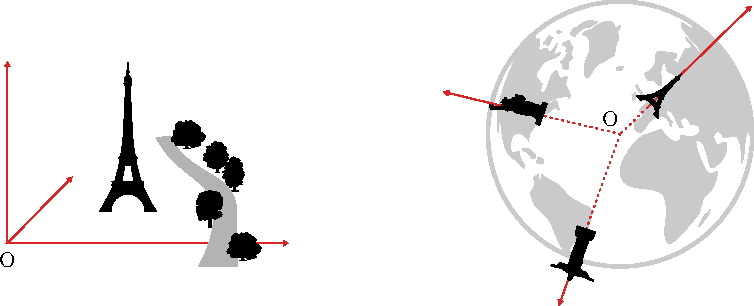
\includegraphics[width=.6\linewidth]{ref_ter}
			      \captionof{figure}{Référentiels terrestres}
		      \end{center}
		\item[b]{Référentiel géocentrique}~:
		      \begin{itemize}
			      \item[b]{Origine}~: \psw{O le centre de la Terre}
			      \item[b]{Axes}~: \psw{3 axes vers des \textbf{étoiles lointaines}
				            fixes}
			      \item[b]{Utilité}~: \psw{étude des satellites de la Terre}
		      \end{itemize}
		      \begin{center}
			      \fatbox{\textbf{Un objet fixe à la surface de la Terre se déplace
					      dans ce référentiel}.}
		      \end{center}
		\item[b]{Référentiel héliocentrique}~:
		      \begin{itemize}
			      \item[b]{Origine}~: \psw{O le centre du \textbf{Soleil}}
			      \item[b]{Axes}~: \psw{3 axes vers des \textbf{étoiles lointaines}
				            fixes}
			      \item[b]{Utilité}~: \psw{étude du mouvement des planètes du système
				            solaire}
		      \end{itemize}
		      \begin{center}
			      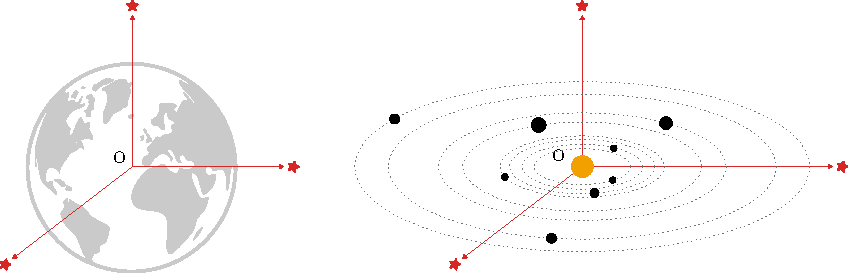
\includegraphics[width=.7\linewidth]{ref_geo-helio}
		      \end{center}
	\end{itemize}
\end{tcb*}

\begin{tcb}[breakable](exem)<lftt>{Importance du référentiel}
	\begin{itemize}
		% \item Une personne dans un train est immobile du point de vue de la
		% personne assise à côté, alors que du point de vue du quai, elle est en
		% translation.
		\item Du point de vue d'um cycliste, la valve de sa roue est en rotation
		      autour de l'axe de la roue. Selon um passant-e immobile, elle suit un
		      mouvement de cycloïde. Son altitude atteint $0$ à chaque tour de roue.
		      \begin{center}
			      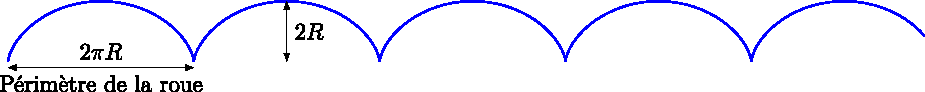
\includegraphics[width=\linewidth]{roue}
		      \end{center}
		\item Du point de vue d'um terrien-ne fixe sur Terre (référentiel
		      terrestre), un arbre planté ne bouge pas. Du point de vue du centre de la
		      Terre (référentiel géocentrique), il tourne à la vitesse vertigineuse de
		      \xul{\psw{\SI{1100}{km.h^{-1}}}}.
	\end{itemize}
\end{tcb}

\begin{tcb}(rema)<lftt>{Mécanique relativiste}
	Nous resterons cette année en mécanique \textbf{classique}, c'est-à-dire que
	les corps étudiés auront une vitesse très inférieure à celle de la lumière
	dans le vide~:
	\psw{%
		\[
			v \ll c = \SI{3.00e8}{m.s^{-1}}
		\]
	}%
	Ce faisant, les mesures de longueurs ou de durées seront
	\textbf{absolues} et indépendantes du référentiel. Ça n'est pas le cas en
	mécanique \textit{relativiste}~: il faut alors ajouter une \textbf{horloge
		interne} au référentiel pour prendre en compte les effets de dilatation du
	temps.
\end{tcb}

\begin{tcb}[breakable](exem)<lftt>{Exemple d'effet relativiste}
	En plus de sa lumière, le Soleil émet plein de particules. Parmi elles se
	trouvent les \textbf{muons}. On peut en recréer en laboratoire et mesurer leur
	durée de vie dans l'atmosphère~; on trouve alors
	\psw{%
		\[
			\tau\ind{labo} = \SI{2.0}{\micro s}
		\]
	}%
	\begin{isd}[interior hidden](exem)
		Ainsi, même en allant à la vitesse de la lumière, leur distance de parcours
		attendue $d$ dans l'atmosphère d'épaisseur $h$ serait de~:
		\psw{%
			\[
				d = c\tau\ind{labo} = \SI{600}{m} \ll h = \SI{600}{km}
			\]
		}%
		Or, \textbf{on détecte de nombreux muons au sol}~! Dans le cadre de la
		mécanique classique, ils devraient aller à une vitesse \textbf{supérieure à la
			célérité de la lumière dans le vide}, ce qui est prohibé par la théorie.
		\tcblower
		\begin{center}
			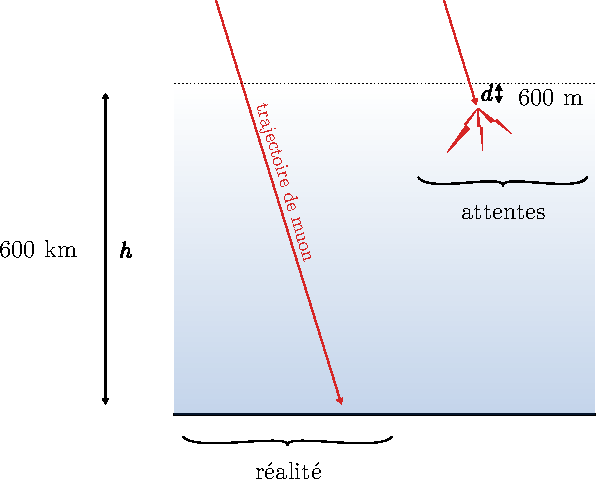
\includegraphics[width=\linewidth]{relat_rst}
		\end{center}
	\end{isd}
	Il s'opère en réalité une \textbf{dilatation de son temps de vie} pour um
	observataire extérieurx en fonction de sa vitesse~:
	\psw{%
		\[
			\tau\ind{propre} = \gamma\,\tau\ind{labo}
			\qav
			\gamma = \frac{1}{\sqrt{1-\dfrac{v^2}{c^2}}}
			\quad \Ra \quad
			\xul{\tau\ind{propre} = \SI{82}{\micro s}}
			\quad \Ra \quad
			\xul{d\ind{réelle} = \SI{27.0}{km}}
		\]
	}%
	\vspace{-25pt}
\end{tcb}

\subsection{Outils mathématiques}
\subsubsection{Vecteur}

% Pour décrire le mouvement d'un point dans l'espace, il est nécessaire d'utiliser
% des vecteurs.

\begin{tcb}(rapp){Vecteur}
	Un vecteur est un objet mathématique qui se dénote avec une flèche vers la
	droite au-dessus d'une lettre~: $\vec{\cdot}$, et ayant~:\smallbreak
	\begin{minipage}{0.40\linewidth}
		\begin{itemize}
			\item
			      \psw{%
				      Un \textbf{point d'application}~;
			      }
			\item
			      \psw{%
				      Une \textbf{direction}~;
			      }
		\end{itemize}
	\end{minipage}
	\begin{minipage}{0.50\linewidth}
		\begin{itemize}
			\item
			      \psw{%
				      Un \textbf{sens}~;
			      }
			\item
			      \psw{%
				      Une distance appelée \textbf{norme}, notée $\norm{\vec{\cdot}}$.
			      }
		\end{itemize}
	\end{minipage}
	\begin{framed}
		\centering
		\psw{%
			\textbf{Une} égalité de vecteurs $\Ra$ \textbf{trois} égalités de
			scalaires, une pour chaque direction de l'espace.%
		}
	\end{framed}
\end{tcb}

\subsubsection{Base de projection}

En plus du repère générique du référentiel, il faut choisir un
\textbf{repère spécifique} à l'étude du problème.

\begin{tcb*}(defi){Base de projection et repère}
	On construit le repère spécifique à l'aide d'une \textbf{origine} et d'une
	\textbf{base de projection orthonormée directe}, constituée de 3
	vecteurs tels que~:
	\smallbreak
	\begin{isd}[righthand ratio=.20]
		\begin{itemize}
			\item[b]{Ortho}~: \psw{les trois vecteurs sont orthogonaux
				      entre eux~;}
			\item[b]{Normée}~: \psw{%
				      leur norme est égale à 1\ftn{On dit qu'ils sont
					      \textit{unitaires}.}~;
			      }%
			\item[b]{Directe}~: \psw{%
				      ils respectent la \textbf{règle de la main droite} (chaque
				      vecteur est égal au produit vectoriel des deux précédents).
			      }%
		\end{itemize}
		\tcblower
		\begin{center}
			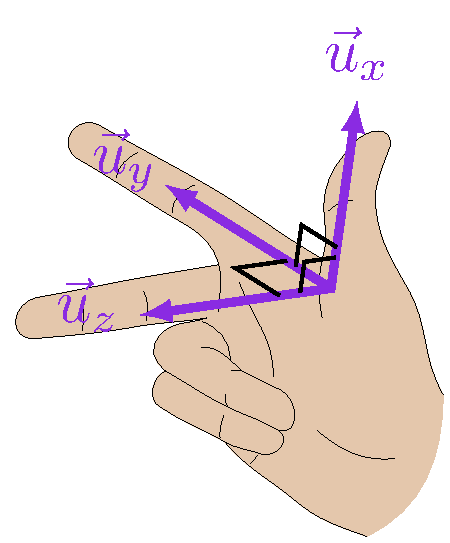
\includegraphics[width=.8\linewidth]{righthand}
			% \captionsetup{justification=centering}
			% \captionof{figure}{}
			% \captionof{figure}{\\Main droite}
		\end{center}
	\end{isd}
	Les vecteurs de base n'ont \textbf{pas d'unité}. Ils définissent les trois
	directions dans lesquelles le point M pourrait se mouvoir.
\end{tcb*}

\begin{tcb}(nota)<lftt>{Vecteur colonne ou explicite}
	Ainsi pour une base générique $(\vv{i}, \vv{j}, \vv{k})$, on
	représente de manière équivalente un vecteur par ses composantes sur chaque
	vecteur de base exprimées en colonne, ou par sa représentation explicite en
	fonction desdits vecteurs de base~:
	\[
		\vv{A} = \mqty(a_i\\a_j\\a_k)
		\Lra
		\vv{A} = a_i \vv{i} + a_j \vv{j} + a_k \vv{k}
	\]
\end{tcb}

\begin{tcb}[breakable](impo){Différence référentiel/repère}
	Il ne faut pas confondre le \textbf{référentiel}, c'est-à-dire le système de
	référence (notion \textit{physique}) avec le \textbf{repère}, c'est-à-dire
	l'outil géométrique qui sert à décrire le mouvement (notion
	\textit{mathématique}). Il y a une infinité de repères spécifiques différents
	qui peuvent être associés à un même référentiel.
\end{tcb}

\subsubsection{Repère fondamental cartésien}

\begin{tcb}[sidebyside, righthand ratio=.25](defi){Repère cartésien}
	Le repère cartésien est constitué d'une origine O autour de laquelle sont
	définis trois vecteurs~:
	\begin{center}
		\psw{%
			$\ux$, $\uy$ et $\uz$ de \textbf{direction constante dans le temps}\ftn{On
				trouve parfois la notation $\ex$, $\ey$, $\ez$.}.
		}%
	\end{center}
	Jusqu'à notifié autrement, ce sera notre repère de prédilection.
	\tcblower
	\begin{center}
		\sswitch{%
			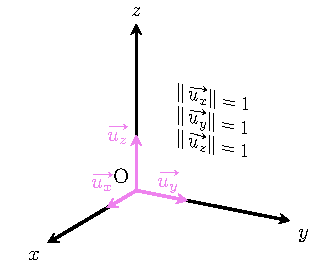
\includegraphics[width=\linewidth, draft=true]{cart}
		}{%
			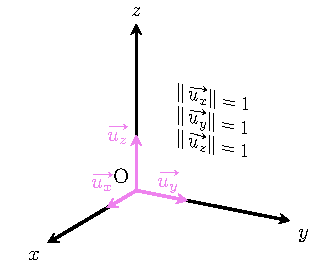
\includegraphics[width=\linewidth]{cart}
		}%
		\captionsetup{justification=centering}
		\captionof{figure}{\\Repère cartésien.}
	\end{center}
\end{tcb}

\subsection{Projection d'un vecteur sur un autre}
On aura souvent des vecteurs définis par une \textbf{norme} et un \textbf{angle}
par rapport à l'un des axes, et l'on souhaiterait obtenir sa décomposition dans
la base de projection.
\begin{tcb*}[sidebyside, righthand ratio=.3](tool){Projection vectorielle (2D)}
	Pour déterminer les coordonnées d'un vecteur $\vv{A}$ sur les vecteurs de base
	d'un repère, on réalise une \textbf{projection}~:
	\psw{%
		\[
			\vv{A}\!\cdot\!\!\ux = A_x
			\qet
			\vv{A}\!\cdot\!\!\uy = A_y
		\]
	}%
	On peut alors utiliser les propriétés du produit scalaire~:
	\psw{%
		\[
			\vv{A}\cdot \vv{B} = \norm{\vv{A}}\norm{\vv{B}}\cos(\theta)
		\]
	}%
	avec $\th$ l'angle entre les vecteurs, pris \textbf{positivement en sens
		trigonométrique}.
	% \bigbreak
	% On pourra également trouver les dépendances des composantes selon cosinus ou
	% sinus par des tests de vraisemblance.
	\tcblower
	\begin{center}
		\sswitch{
			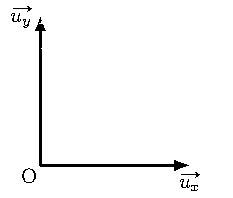
\includegraphics[width=\linewidth]{proj_stud}
		}{
			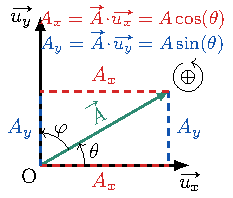
\includegraphics[width=\linewidth]{proj_prof}
		}
		\vspace{-15pt}
		\captionof{figure}{Projection 2D}
	\end{center}
\end{tcb*}

\section{Position, vitesse et accélération}
\subsection{Position}
\subsubsection{Définition}

\begin{tcb}[sidebyside, righthand ratio=.25](defi){Position en cartésiennes}
	On note la postion $\OM(t)$, \textbf{homogène à une distance}. Elle s'exprime
	\[\psw{\boxed{\OM(t) = x(t)\ux + y(t)\uy + z(t)\uy}}\]
	et sa \textbf{norme} se calcule avec~:
	\[\psw{\boxed{\OMr(t) = \norm{\OM(t)} = \sqrt{x(t)^2 + y(t)^2 + z(t)^2}}}\]
	\tcblower
	\begin{center}
		\sswitch{
			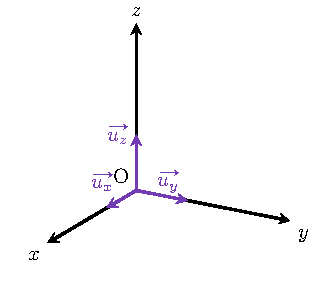
\includegraphics[width=\linewidth]{pos_cart_stud}
		}{
			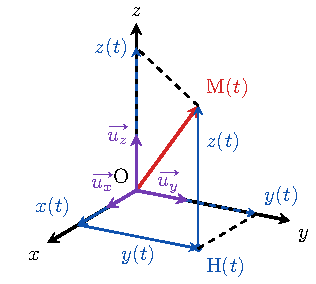
\includegraphics[width=\linewidth]{pos_cart_prof}
		}
		\vspace{-15pt}
		\captionsetup{justification=centering}
		\captionof{figure}{\\Position cartésienne.}
	\end{center}
\end{tcb}

\subsubsection{Déplacement élémentaire}
\begin{tcb}[sidebyside, righthand ratio=.35](defi){Déplacement élémentaire
			cartésien}
	Le \textbf{déplacement élémentaire} est le déplacement infiniment petit du
	point M pendant un temps infinitésimal $\dt$. En cartésiennes,
	\psw{%
		\begin{gather*}
			\OM(t) = \mqty(x(t)\\y(t)\\z(t))
			\to
			\OM(t+\dt) = \mqty(x(t)+\dd{x}\\y(t)+\dd{y}\\z(t)+\dd{z})
			\\\Ra
			\boxed{\dd\OM = \OM(t+\dt)-\OM(t) = \dd{x}\ux + \dd{y}\uy + \dd{z}\uz}
		\end{gather*}
	}%
	\vspace{-15pt}
	\tcblower
	\begin{center}
		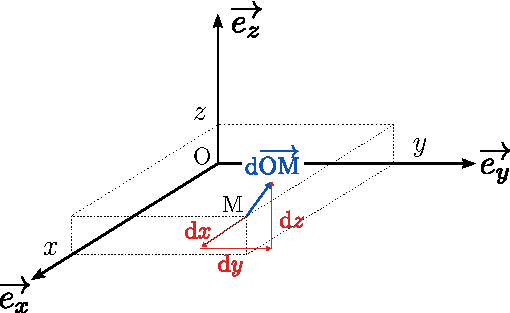
\includegraphics[width=\linewidth]{dOM_cart}
		% \sswitch{
		% 	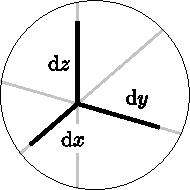
\includegraphics[width=\linewidth, draft=true]{delem_cart}
		% }{
		% 	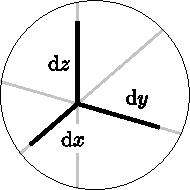
\includegraphics[width=\linewidth]{delem_cart}
		% }
		% \vspace{-15pt}
		\captionsetup{justification=centering}
		\captionof{figure}{\\$\dd{\protect\OM}$ en cartésiennes.}
	\end{center}
\end{tcb}

\subsubsection{Équations horaires et trajectoire}
\begin{tcb}(defi)<lftt>{Équations horaires}
	Les \textbf{équations horaires} du mouvement sont les fonctions $x(t)$,
	$y(t)$ et $z(t)$ exprimées \textbf{explicitement} en fonction du temps $t$.
\end{tcb}

\begin{tcb}(exem)<lftt>{Équations horaires en TP}
	\begin{center}
		\begin{tabularx}{\linewidth}{Y|Y|Y}
			\textbf{Chute dans glycérol}
			 &
			\textbf{Chute libre verticale}
			 &
			\textbf{Chute libre $\vf(0) = v_0\ux$}
			\\
			\begin{center}
				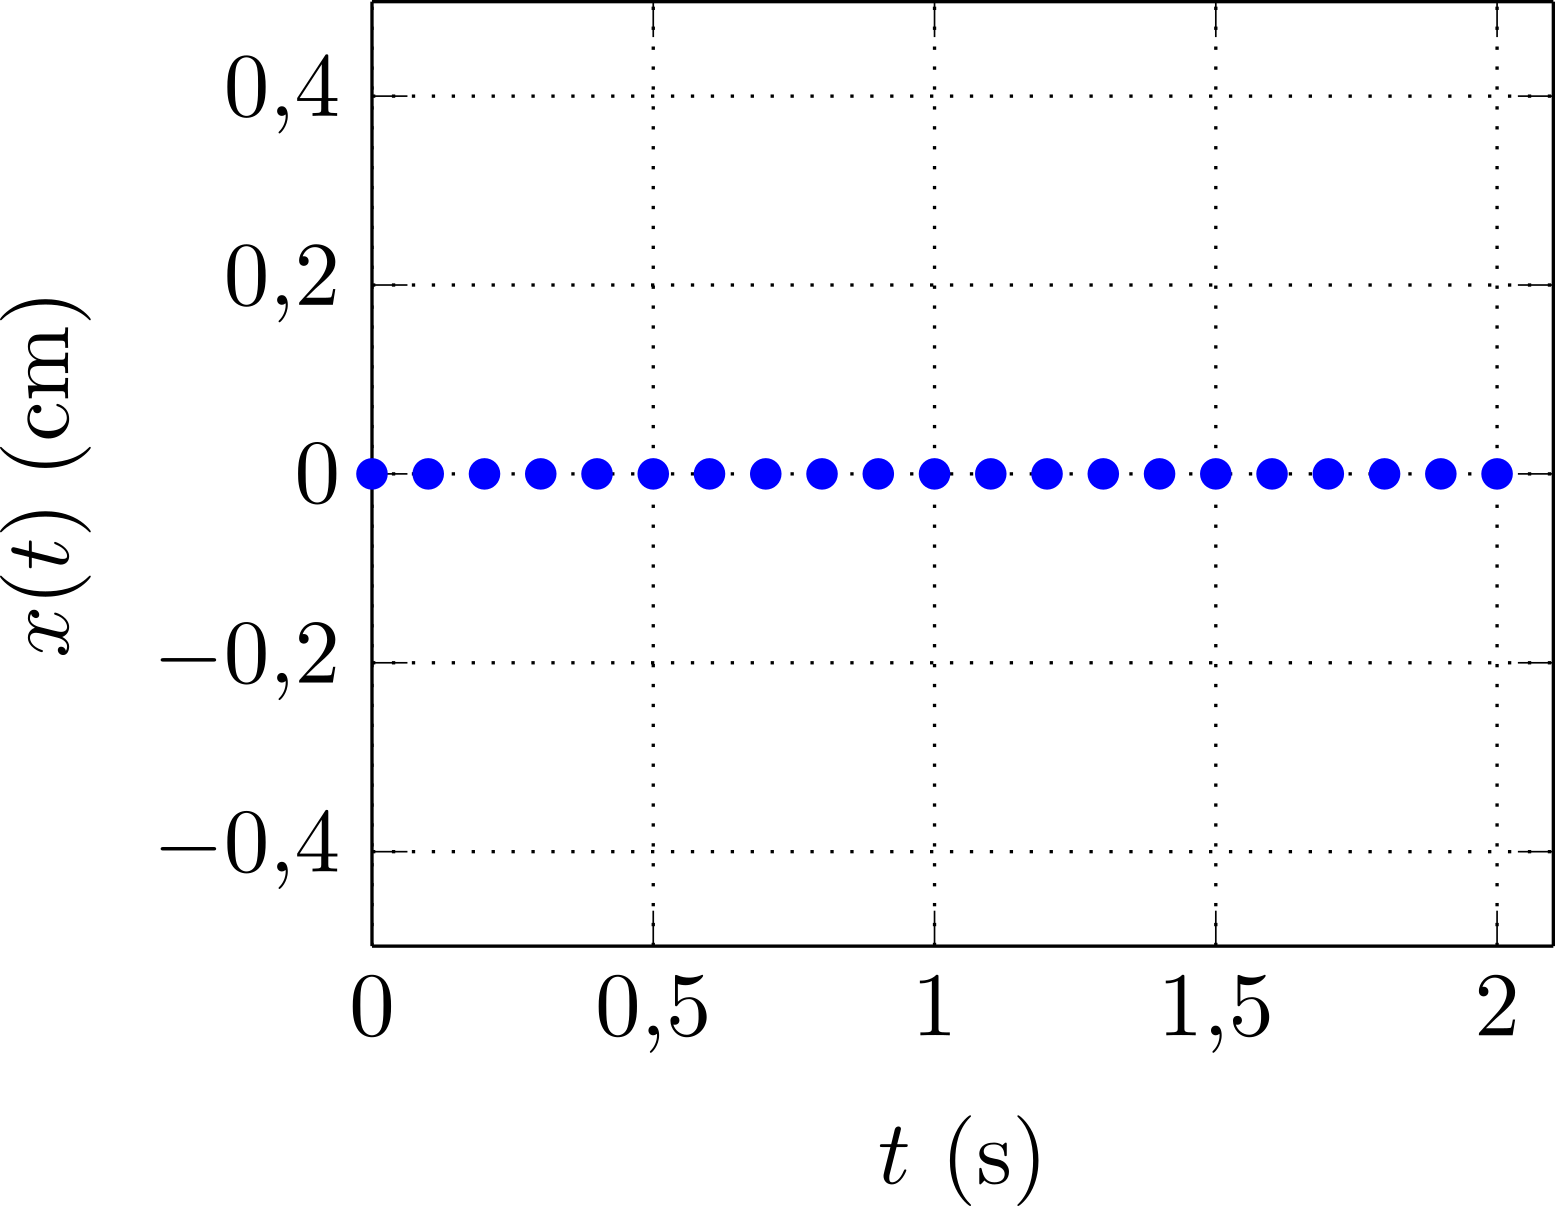
\includegraphics[height=4cm]{x_glyc}
				\\
				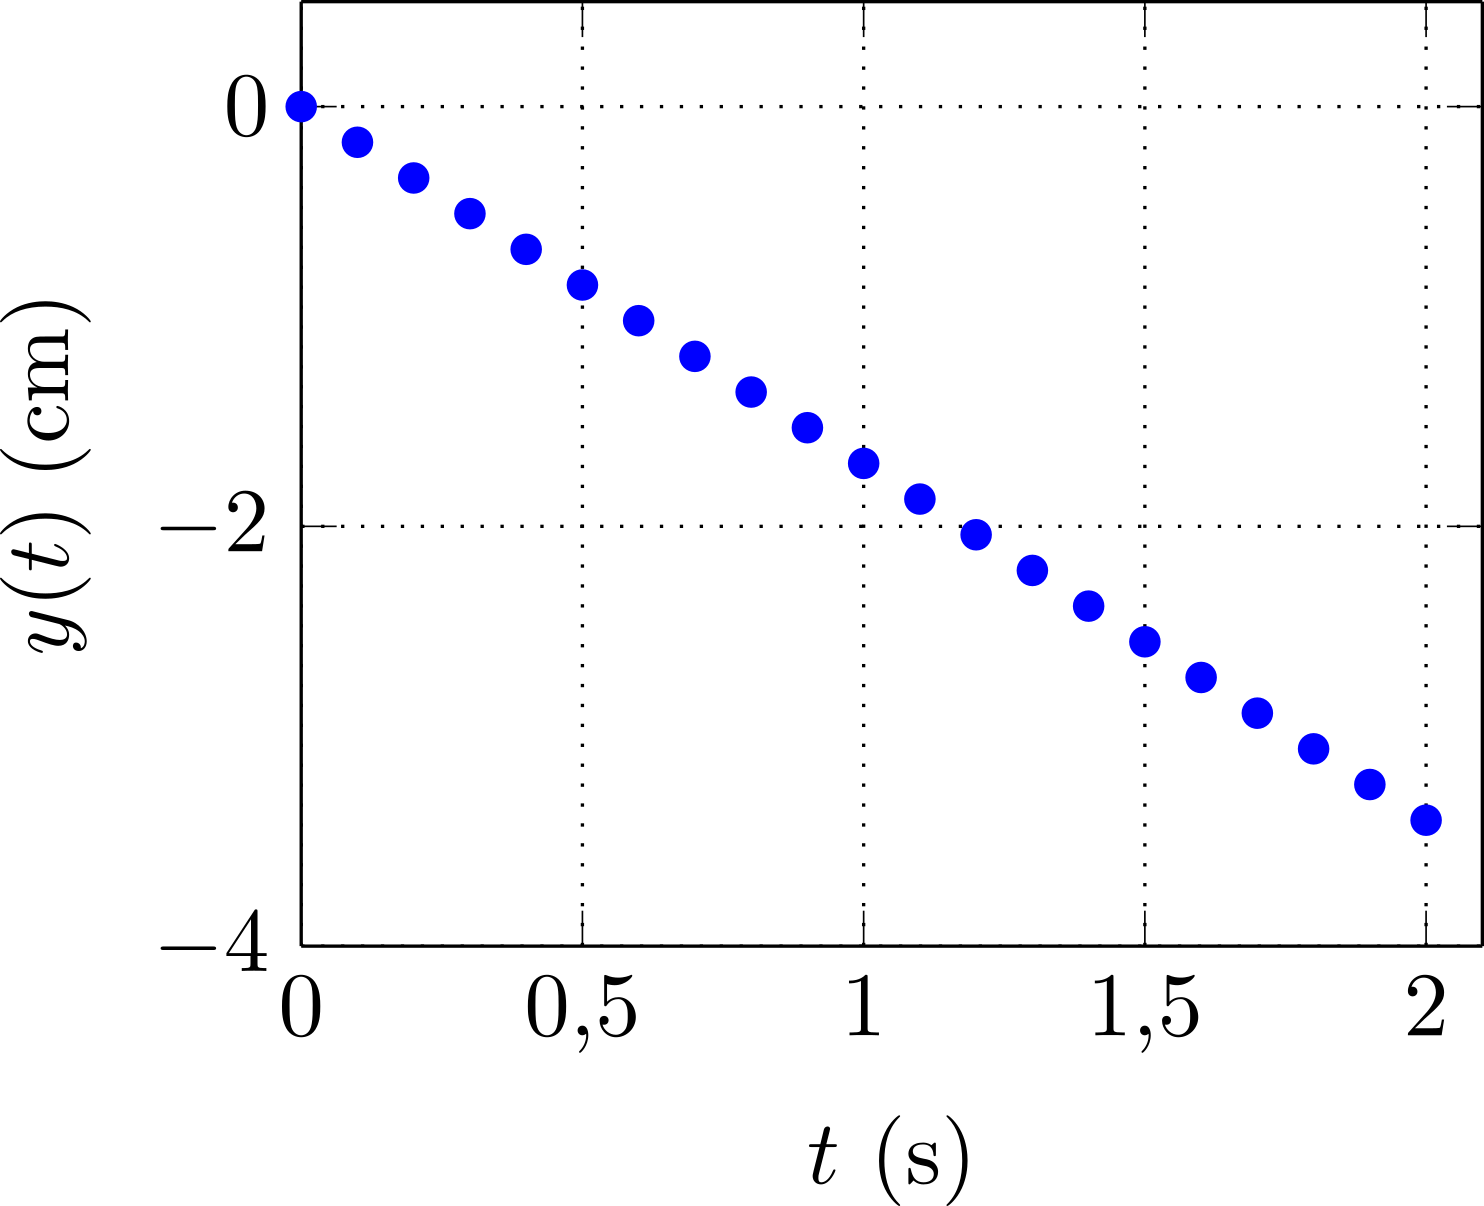
\includegraphics[height=4cm]{y_glyc}%
				\vspace*{-25pt}
			\end{center}
			 &
			\begin{center}
				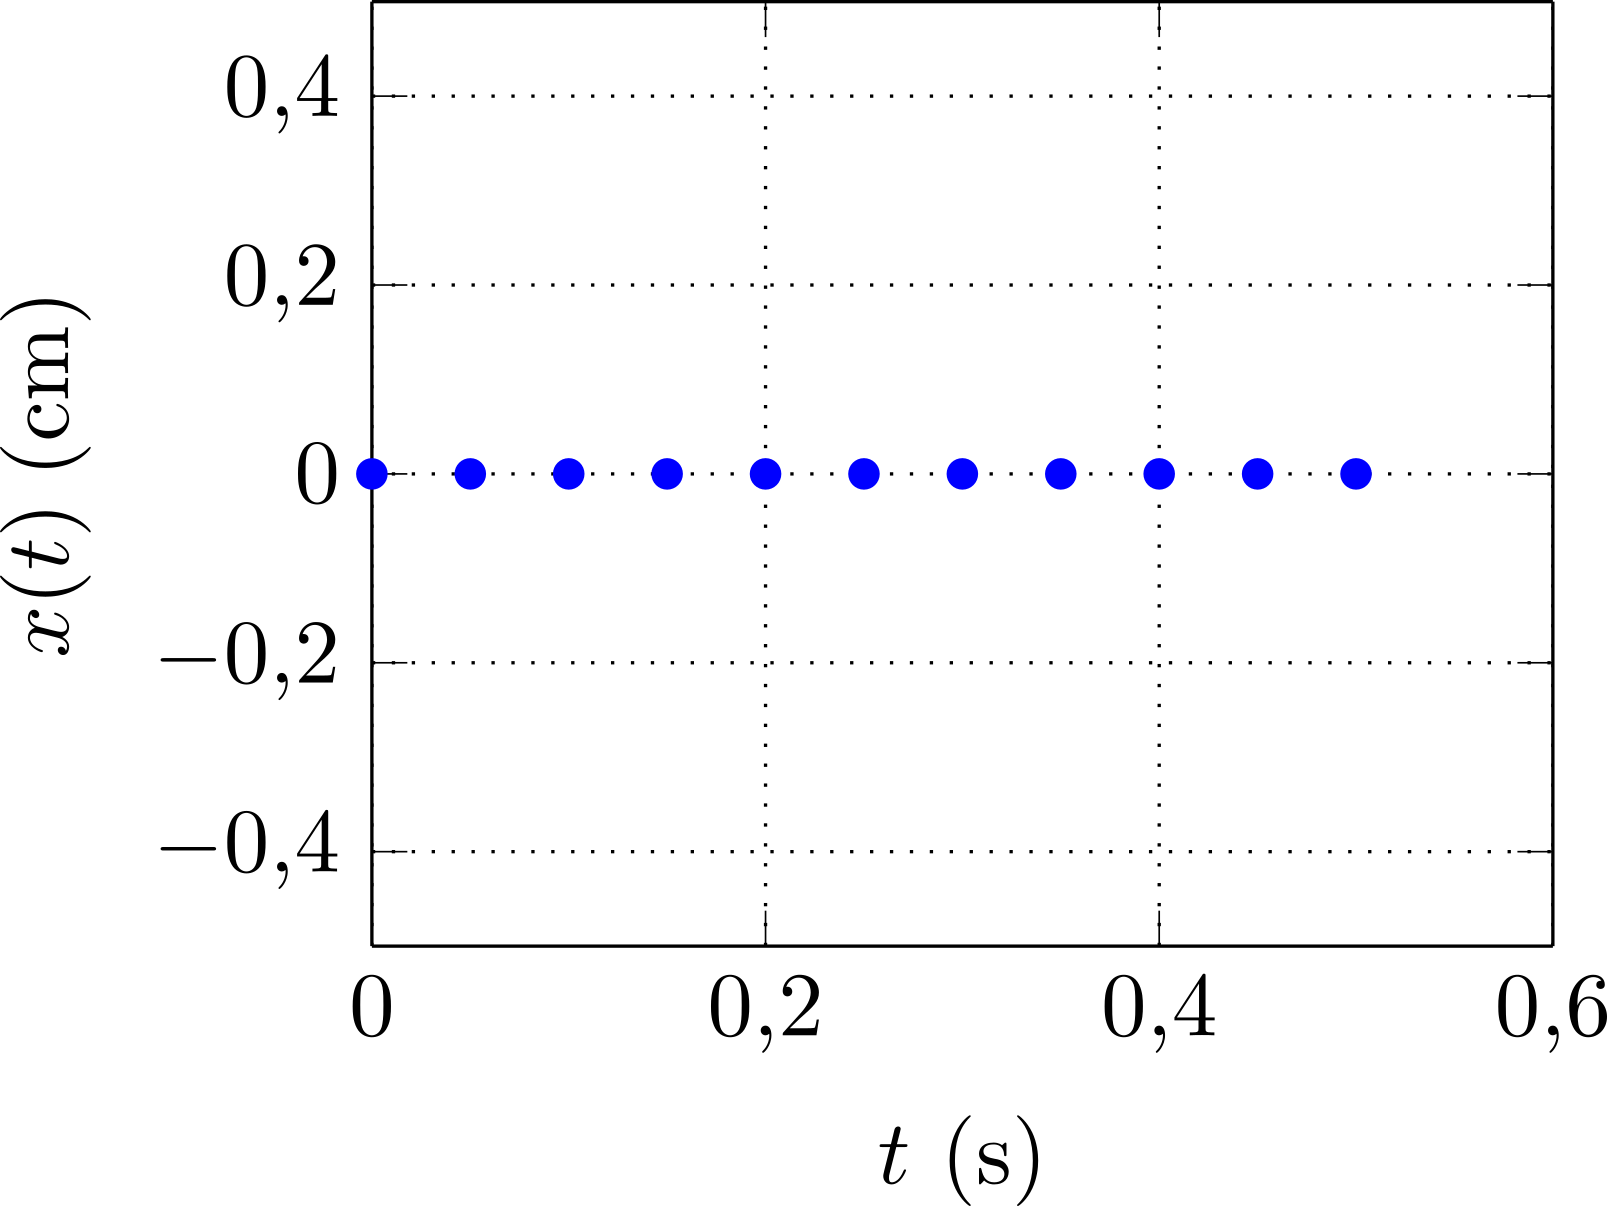
\includegraphics[height=4cm]{x_nov}
				\\
				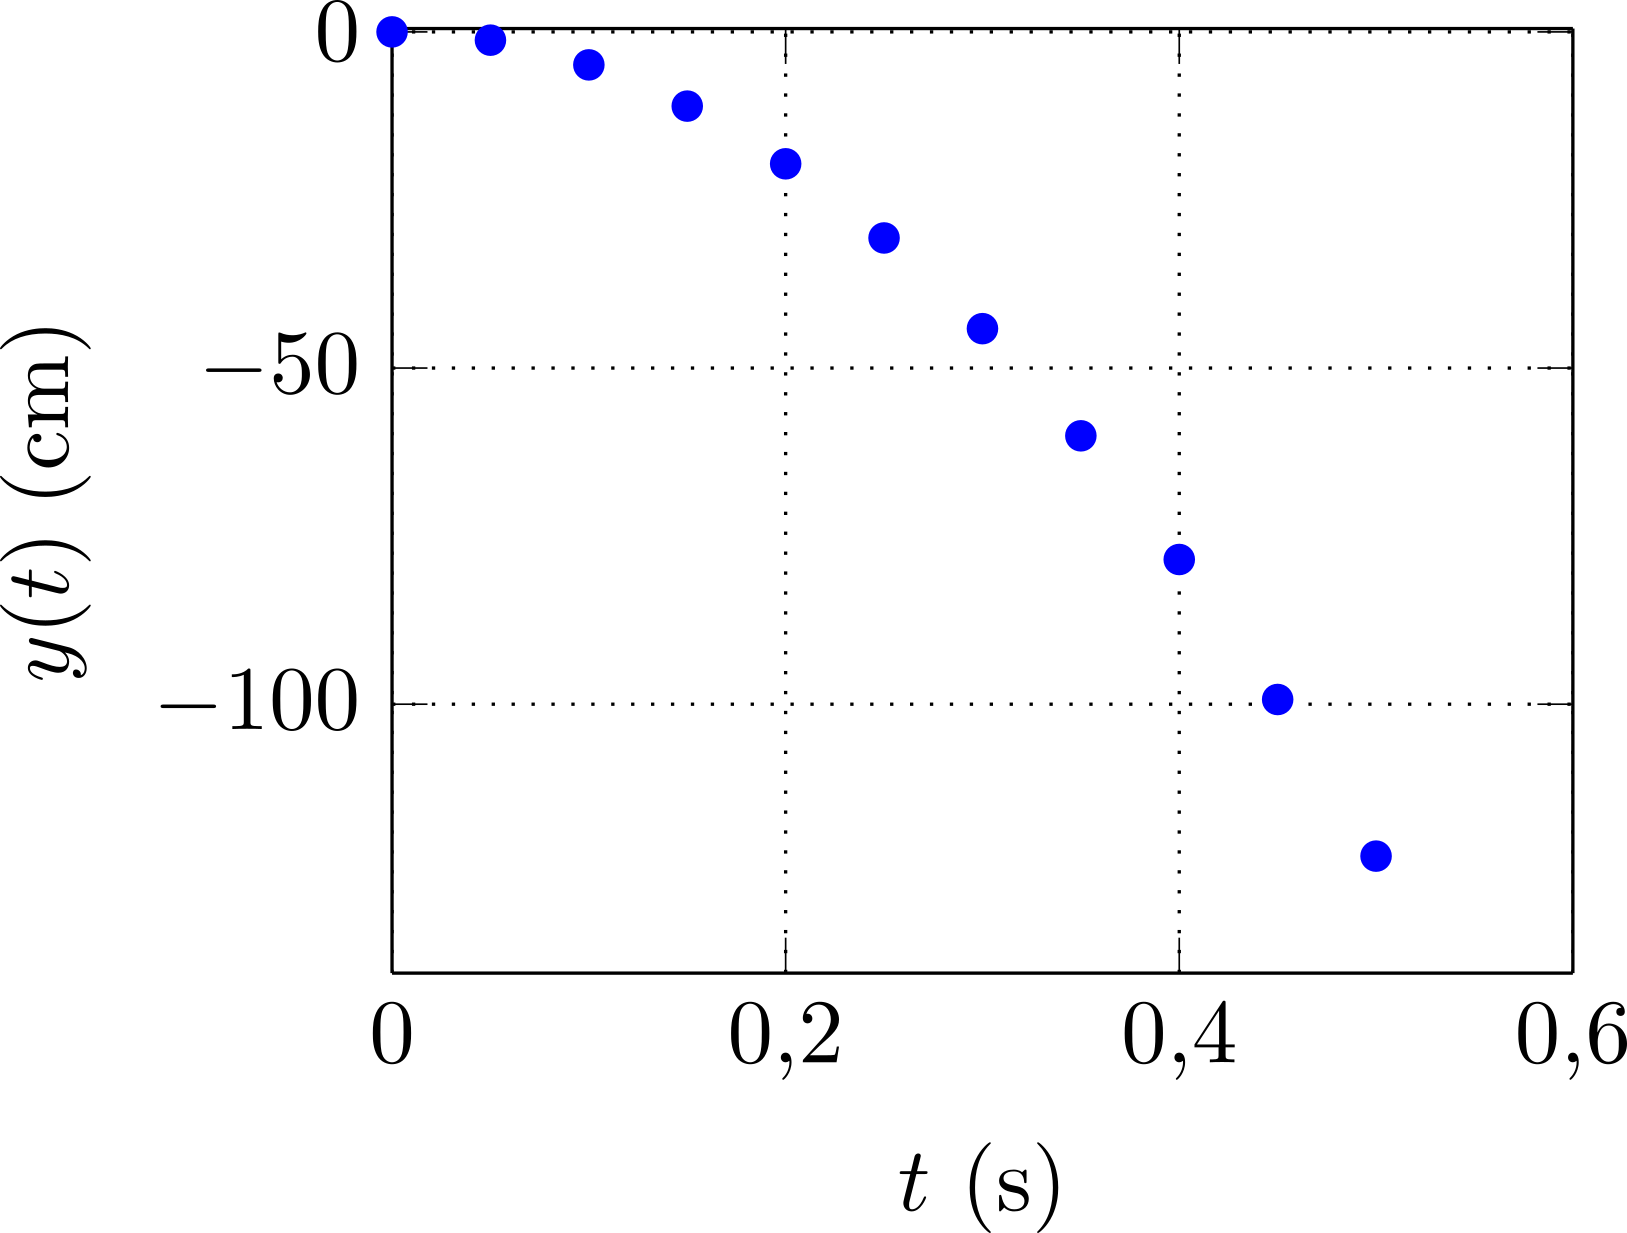
\includegraphics[height=4cm]{y_nov}%
				\vspace*{-25pt}
			\end{center}
			 &
			\begin{center}
				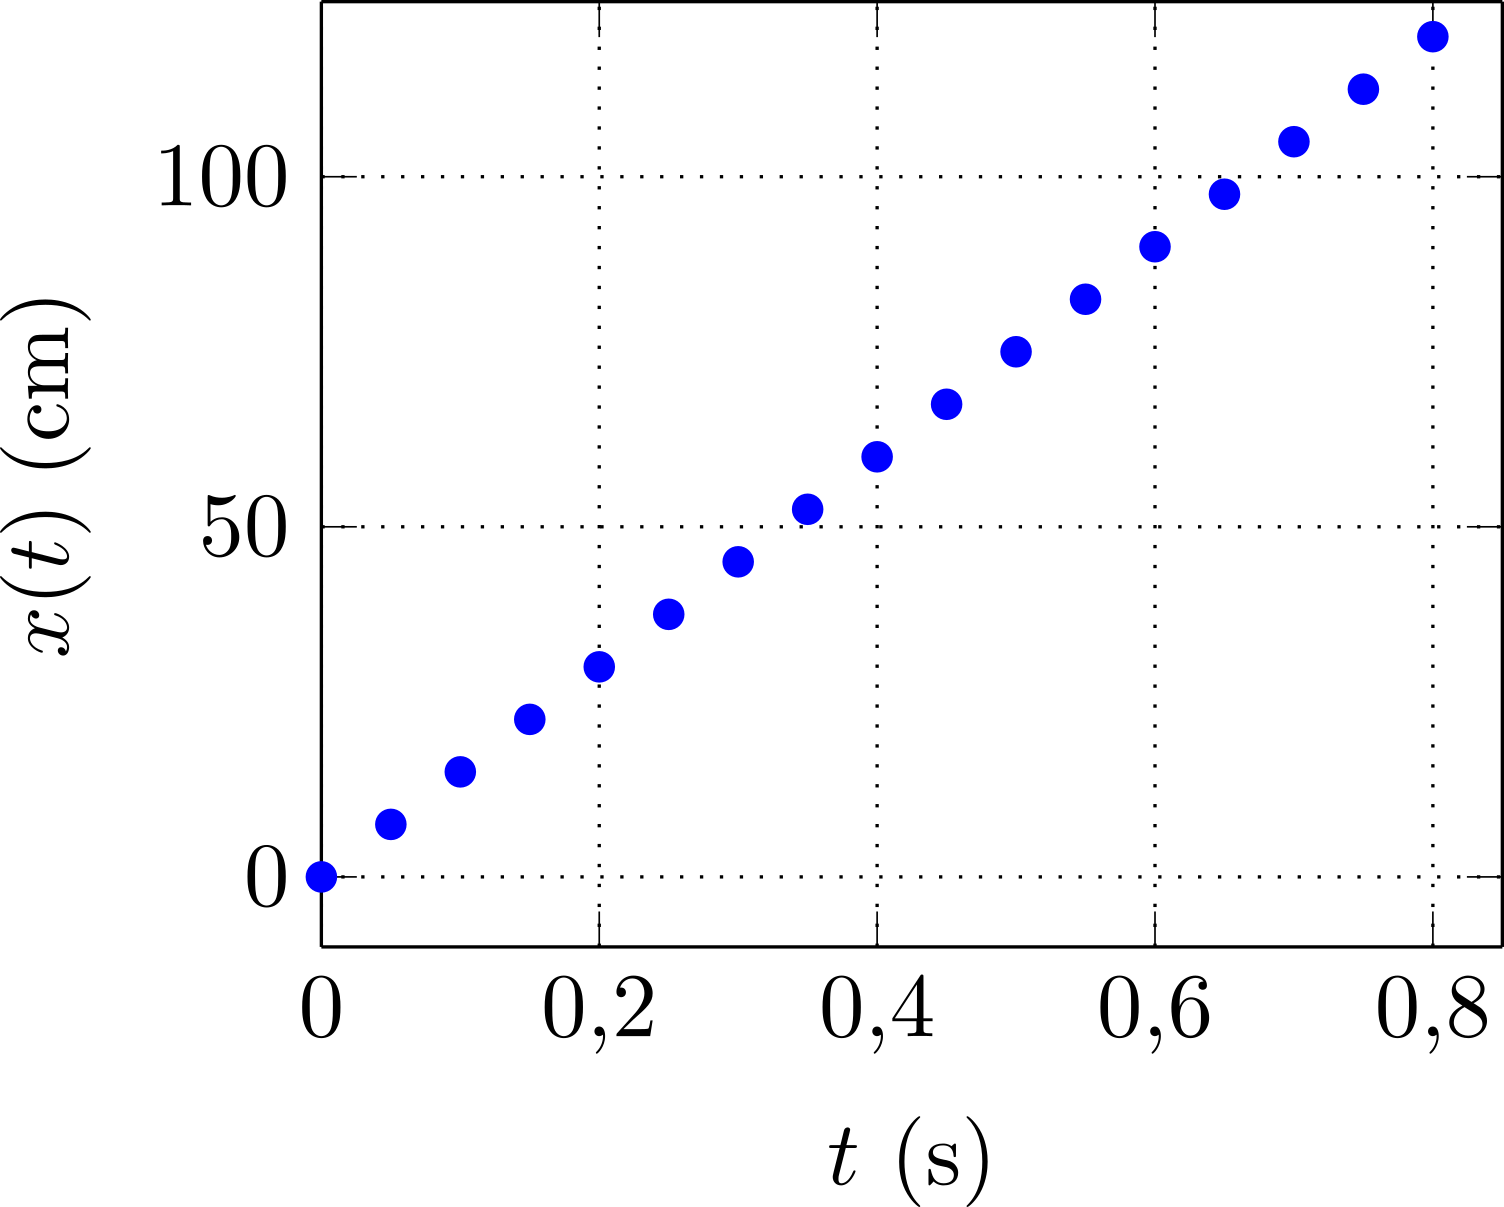
\includegraphics[height=4cm]{x_vo}
				\\
				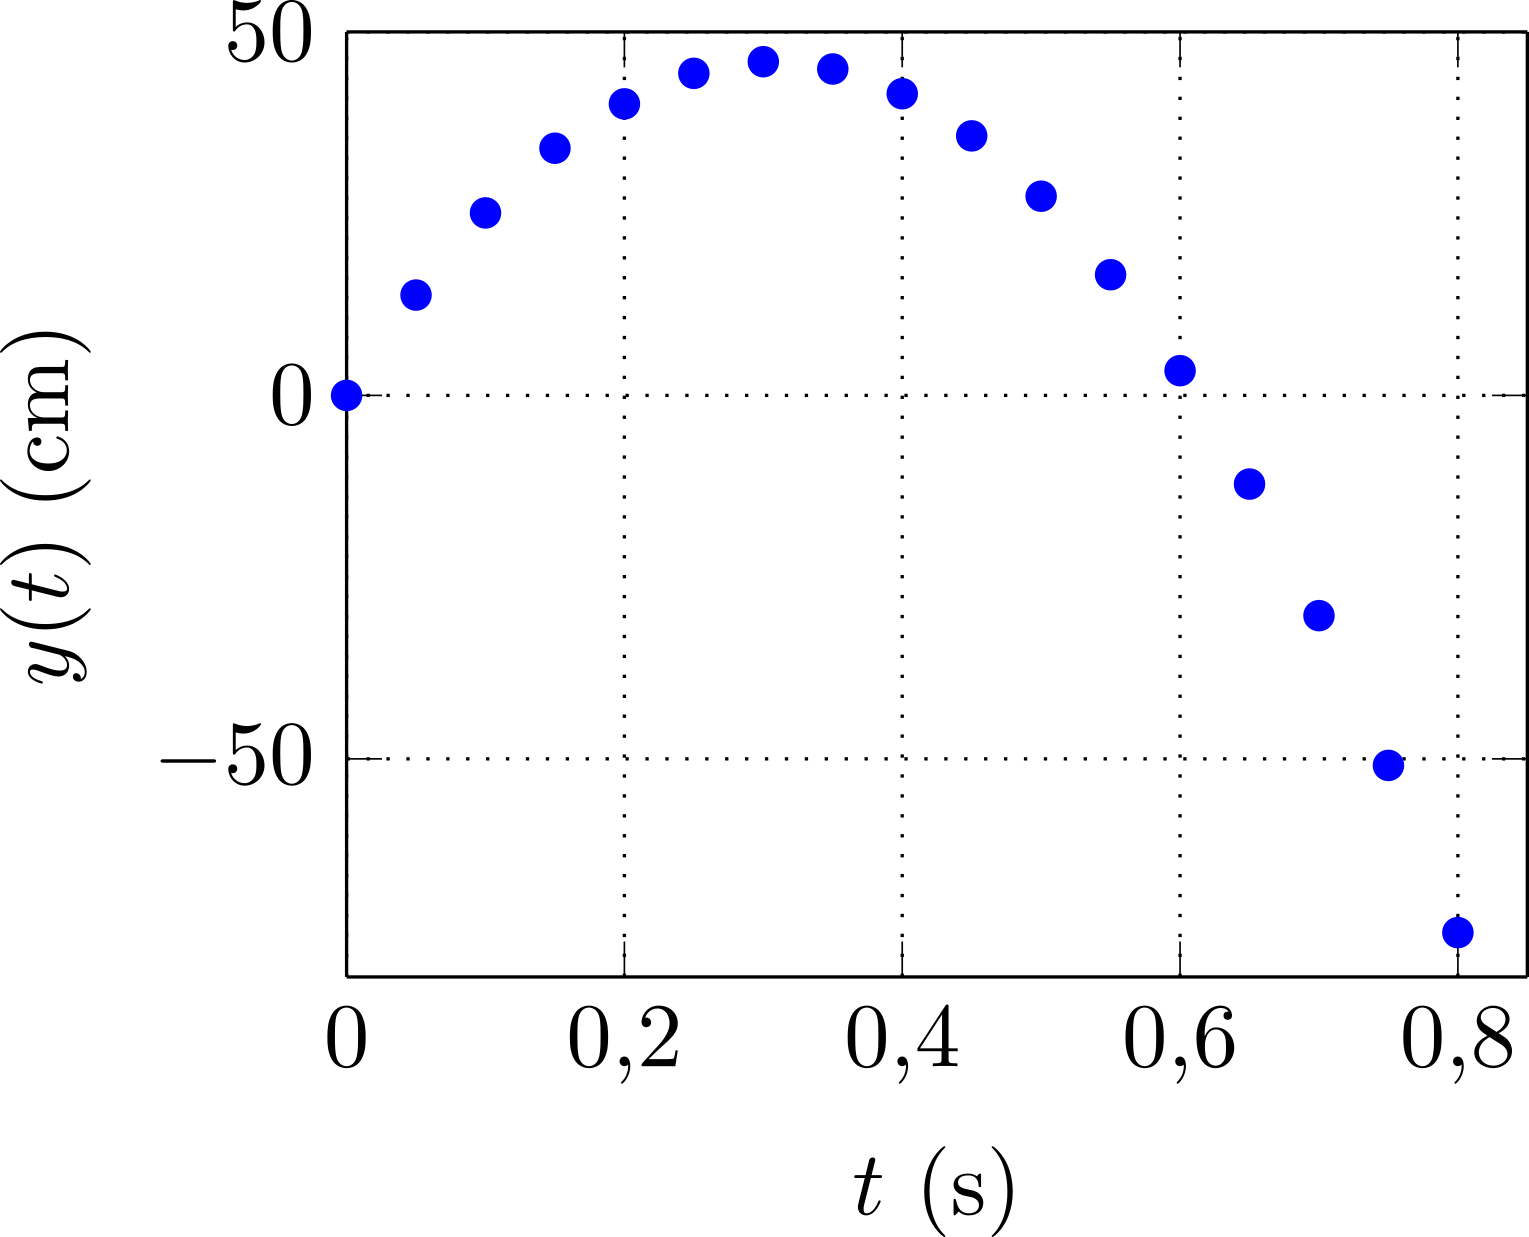
\includegraphics[height=4cm]{y_vo}%
				\vspace*{-25pt}
			\end{center}
		\end{tabularx}
		% \vspace{-15pt}
	\end{center}
\end{tcb}

\begin{tcb}(defi)<lftt>{Trajectoire}
	La \textbf{trajectoire} est l'ensemble des positions successives du point
	M$(t)$ au cours du temps. C'est le «~dessin~» fait par le mobile au cours du
	temps dans l'espace.
\end{tcb}

\begin{tcb}(exem)<lftt>{Trajectoires en TP}
	Sur les exemples précédents, la trajectoire est la courbe $y(x)$ car le
	mouvement est plan. C'est une droite dans les deux premiers cas, et une parabole
	dans le dernier.
	\begin{center}
		\begin{tabularx}{\linewidth}{Y|Y|Y}
			\textbf{Chute dans glycérol}
			 &
			\textbf{Chute libre verticale}
			 &
			\textbf{Chute libre $\vf(0) = v_0\ux$}
			\\
			\begin{center}
				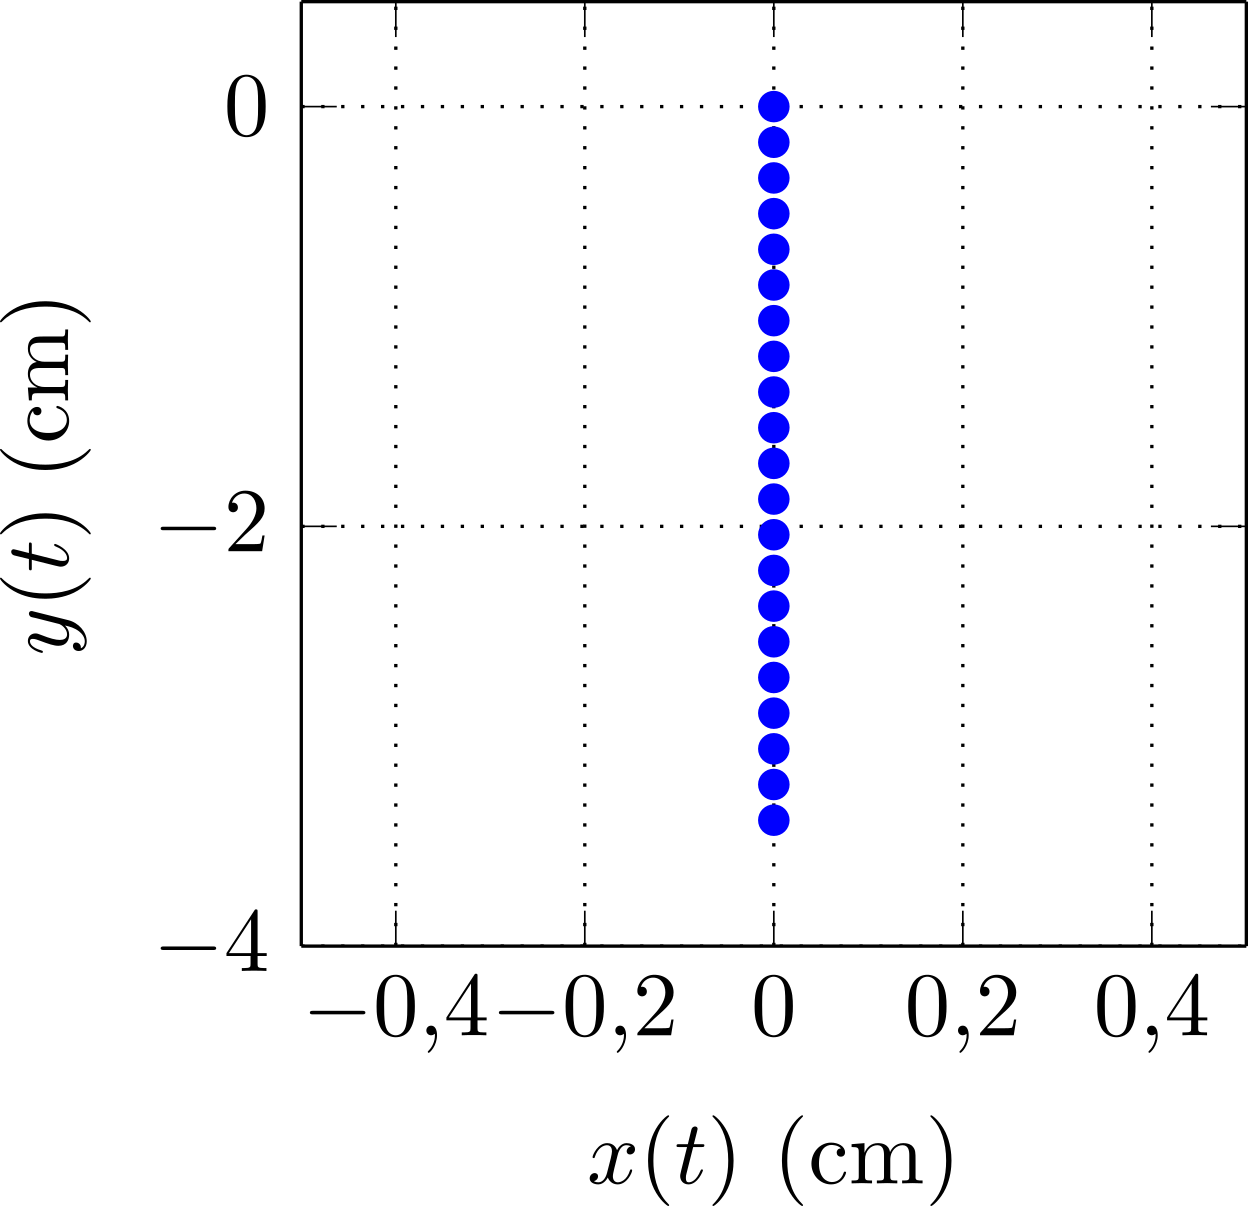
\includegraphics[height=4cm]{traj_glyc}
				\vspace*{-25pt}
			\end{center}
			 &
			\begin{center}
				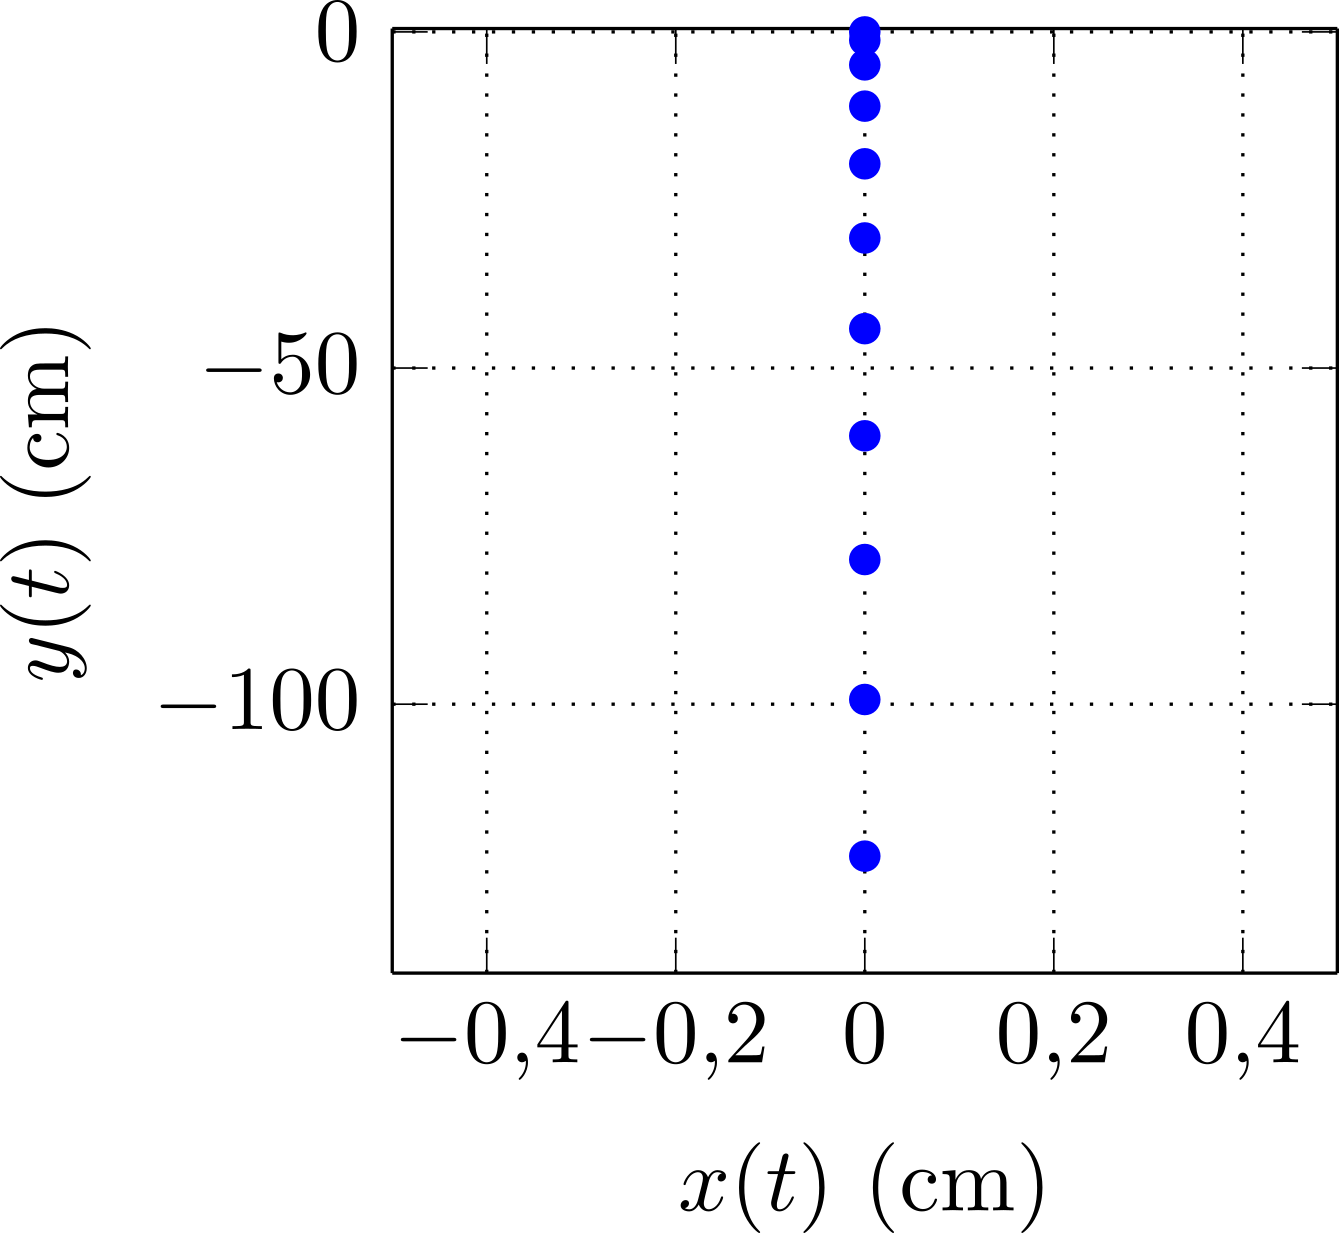
\includegraphics[height=4cm]{traj_nov}
				\vspace*{-25pt}
			\end{center}
			 &
			\begin{center}
				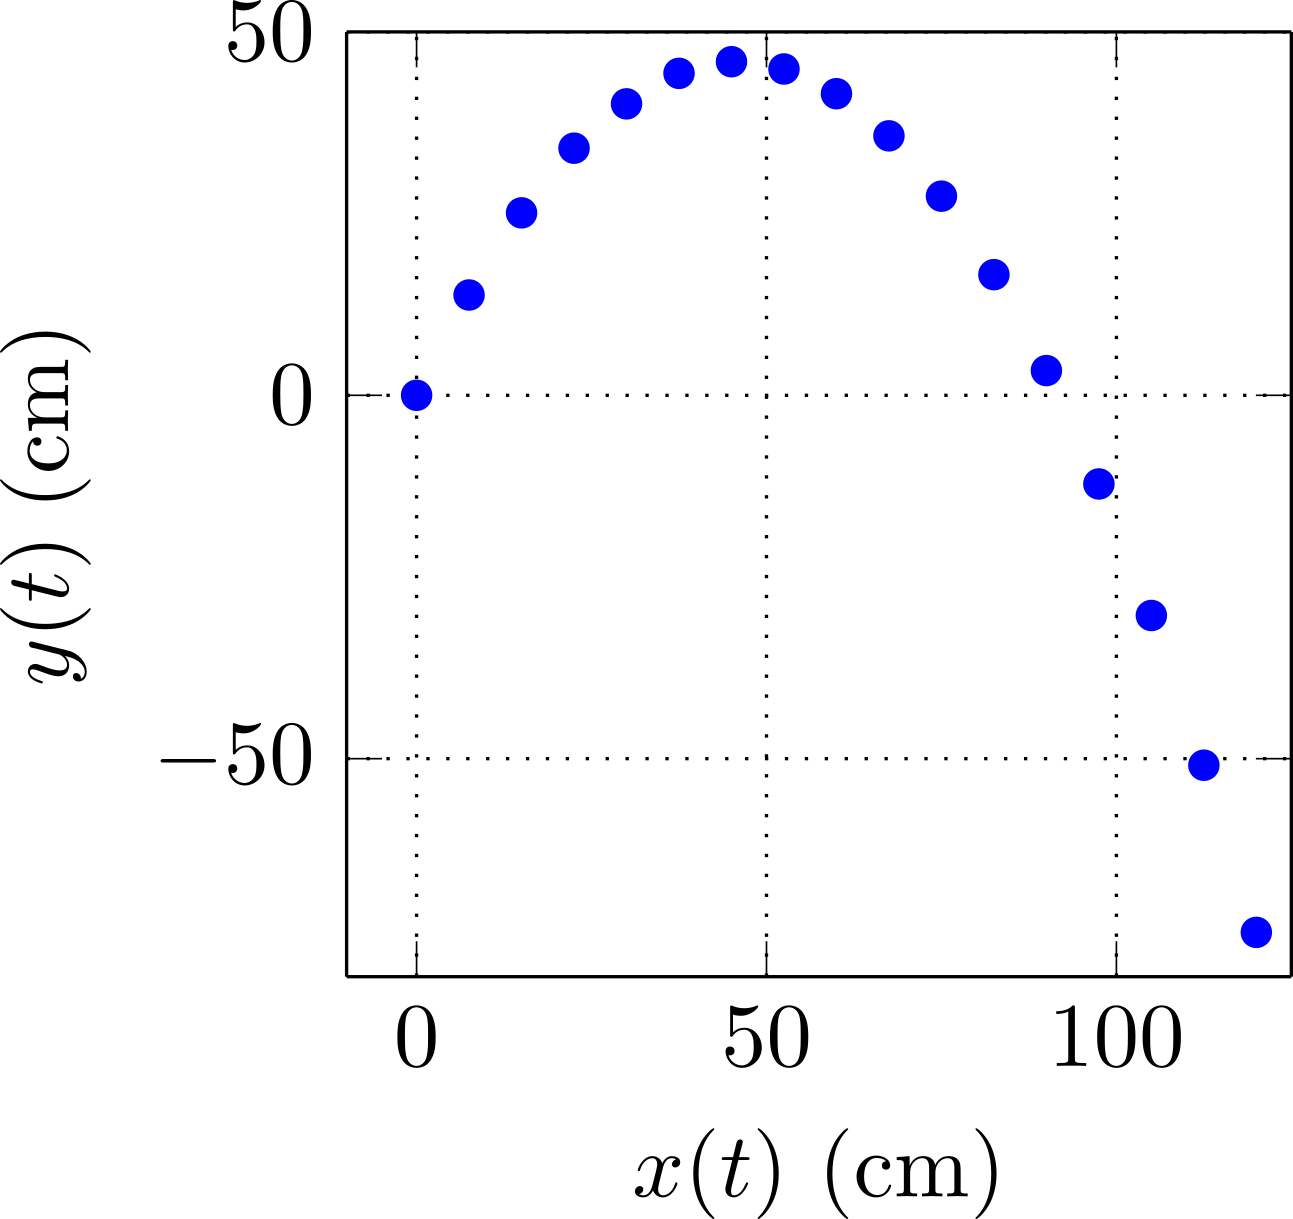
\includegraphics[height=4cm]{traj_vo}
				\vspace*{-25pt}
			\end{center}
		\end{tabularx}
	\end{center}
\end{tcb}

\subsection{Vitesse}
\begin{tcb}[sidebyside, righthand ratio=.25](defi){Vitesse}
	On définit la \textbf{vitesse} comme la \textbf{limite du taux
		d'accroissement} du vecteur position~:
	\[
		\psw{%
			\boxed{%
				\vf(t) =
				\lim_{\Delta{t}\to 0} \frac{\OM(t+\Dt) - \OM(t)}{\Dt} =
				\dv{\OM}{t}
			}%
		}%
		\qdonc
		\psw{[\vf] = \si{m.s^{-1}}}
	\]
	%  Si on effectue des mesures très rapprochées, c'est-à-dire $\Dt \rightarrow
	%    0$, on définit alors la vitesse \textit{instantanée} par~:
	% \[\psw{\boxed{\vf(t) = \dv{\OM(t)}{t}}}\]
	\tcblower
	\begin{center}
		\sswitch{
			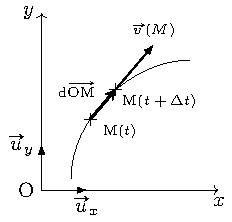
\includegraphics[width=\linewidth, draft=true]{vec_vit}
		}{
			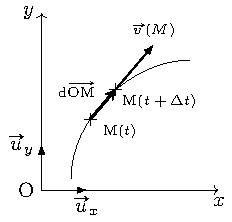
\includegraphics[width=\linewidth]{vec_vit}
		}
		\vspace{-15pt}
		\captionsetup{justification=centering}
		\captionof{figure}{\\Vecteur vitesse.}
	\end{center}
\end{tcb}

\begin{tcb}[cnt, bld](ror){Vitesse et trajectoire}
	Le vecteur vitesse est toujours tangent à la trajectoire.
\end{tcb}

\begin{tcb*}(prop){Vitesse en cartésiennes}
	\psw{%
		\[
			\vf(t) = \xp(t)\ux + \yp(t)\uy + \zp(t)\uz
		\]
	}%
	\vspace{-15pt}
\end{tcb*}

\begin{tcb*}(demo){Vecteur vitesse}
	On peut donc voir la vitesse comme étant le \textbf{rapport entre $\dd{\OM}$
		et $\dd{t}$}, ou comme étant la \textbf{dérivée de $\OM(t)$}. Or, \textbf{les
		vecteurs de la base cartésienne sont constants dans le temps}, soit~:
	\smallbreak
	\begin{isd}[interior hidden](demo)
		\tcbsubtitle{\fatbox{\textbf{Rapport}}}
		\psw{%
			\begin{align*}
				\vf(t) & =
				\dv{\OM}{t} =
				\frac{\dd{x}\ux + \dd{y}\uy + \dd{z}\uz}{\dd{t}}
				\\\Lra
				\Aboxed{%
				\vf(t) & =
					\dv{x}{t}\ux + \dv{y}{t}\uy + \dv{z}{t}\uz
				}
				\qed
			\end{align*}
		}%
		\tcblower
		\tcbsubtitle{\fatbox{\textbf{Dérivée}}}
		\psw{%
			\begin{align*}
				\vf(t) & =
				\dv{t} \pa{x(t)\ux + y(t)\uy + z(t)\uz}
				\\\Lra
				\Aboxed{%
				\vf(t) & =
					\dv{x}{t}\ux + \dv{y}{t}\uy + \dv{z}{t}\uz
				}
				\qed
			\end{align*}
		}%
	\end{isd}
\end{tcb*}

% \begin{tcb}(nota)<lfnt>'l'{Dérivée temporelle en mécanique}
% 	En mécanique, les dérivées \textbf{par rapport au temps} se notent avec un
% 	point sur la fonction~:
% 	\[\dv{x}{t}(t) = \xp(t)\]
% \end{tcb}

\begin{tcb}(exem)<lftt>{Vitesse selon expérience}
	En reprenant les exemples précédents~:
	\begin{itemize}
		\item Pour la chute dans le glycérol, $\xp(t) = 0$ et $\yp(t) = \cte$. Ainsi,
		      $\vf(t)$ est constant, et dirigé vers le bas.
		\item Pour la chute libre sans vitesse initiale, $\xp(t) = 0$ et $\yp(t)$
		      diminue linéairement~: le vecteur vitesse est variable, dirigé vers
		      le bas.
		\item Pour la chute libre avec vitesse initiale, $\xp(t) = \cte$ et $\yp(t)$
		      diminue linéairement~: le vecteur vitesse est variable et change de
		      direction.
	\end{itemize}
\end{tcb}

\begin{tcb}(impo){Différence vecteur/norme}
	Selon le contexte, on fera particulièrement attention à ne pas confondre le
	mot «~vitesse~» avec le \textbf{vecteur} ou avec sa \textbf{norme}. Une
	vitesse, en \textbf{norme}, \textbf{ne peut pas être négative}~; les
	\textbf{composantes} du vecteur vitesse \textbf{peuvent être négatives}.
\end{tcb}

\subsection{Accélération}
% L'accélération est la grandeur physique qui mesure la variation de la vitesse.
\begin{tcb}(defi){Accélération}
	On définit l'\textbf{accélération} comme la \textbf{limite du taux d'accroissement} du vecteur vitesse~:
	\[
		\psw{%
			\boxed{%
				\af(t) =
				\lim_{\Delta{t}\to 0} \frac{\vf(t+\Dt) - \vf(t)}{\Dt} =
				\dv{\vf}{t} =
				\dv[2]{\OM}{t}
			}%
		}%
		\qdonc
		\psw{[\af] = \si{m.s^{-2}}}
	\]
\end{tcb}

\begin{tcb}[cnt, bld](ror){Accélération et trajectoire}
	Le vecteur accélérations est toujours dirigé vers l'intérieur à la
	trajectoire (partie concave).
\end{tcb}

\begin{tcb*}(prop){Accélération en cartésiennes}
	Par distribution de l'opérateur $\dv{t}$, on obtient en cartésiennes
	\[\psw{\boxed{\af(t) = \xpp(t)\ux + \ypp(t)\uy + \zpp(t)\uz}}\]
\end{tcb*}

\begin{tcb}(exem)<lftt>{Accélération selon expérience}
	En reprenant les exemples précédents~:
	\begin{itemize}
		\item Pour la chute dans le glycérol, $\xpp(t)$ et $\ypp(t)$ sont nuls~: le
		      vecteur accélération est nul.
		\item Pour la chute libre sans vitesse initiale, $\xpp(t) = 0$ et $\ypp(t)$
		      est constant~: le vecteur accélération est constant, dirigé vers le
		      bas.
		\item Pour la chute libre avec vitesse initiale, $\xpp(t) = 0$ et $\ypp(t)$
		      est constant~: le vecteur accélération est constant, dirigé vers le
		      bas.
	\end{itemize}
\end{tcb}

\begin{tcb}(impo){Accélération}
	Une accélération peut être négative et peut être nulle~:
	\begin{itemize}
		\item L'accélération étant liée à la \textbf{variation du
			      vecteur vitesse}, si la vitesse diminue, l'accélération peut être
		      négative.
		\item Pour que l'accélération soit nulle, il faut que \textbf{toutes les
			      composantes} de la vitesse soient constantes. Un mouvement peut
		      être à vitesse constante en norme, mais d'accélération non nulle
		      (mouvement circulaire, cf.\ chapitre M3).
	\end{itemize}
\end{tcb}

\section{Exemples de mouvements}

\subsection{Mouvement rectiligne uniforme}
\begin{tcb}(defi)<lftt>{Mouvement rectiligne uniforme}
	Un mouvement est dit \textbf{uniforme} si la \textbf{norme du vecteur vitesse}
	$\norm{\vf}$ est constante ($\Lra \af = \of$). Il est dit \xul{rectiligne} si
	la \xul{trajectoire est une droite}.
\end{tcb}

\begin{tcb*}(appl)<lftt>{Mouvement rectiligne uniforme}
	Montrer qu'un mouvement caractérisé $\vf(t) = v_0\ux$ donne un mouvement
	rectiligne uniforme.
	\tcblower
	\psw{%
		On intègre pour avoir la position~:
		\[
			\OM(t) = v_0\,t \ux + \OM(0)
		\]
		ce qui décrit bien une droite dans l'espace. C'est le cas de la chute dans
		le glycérol.
	}%
\end{tcb*}

\subsection{Mouvement rectiligne uniformément accéléré}
\begin{tcb}(defi)<lftt>{Uniformément accéléré}
	Un mouvement est dit \textbf{uniformément accéléré} si la \textbf{norme du
		vecteur accélération} $\norm{\af}$ est \textbf{constante}.
\end{tcb}

\begin{tcb*}(appl)<lftt>{Mvt. rect. uniformé\mnt\ accéléré}
	Déterminer les équations horaires pour un mouvement uniformément accéléré
	caractérisé par $\af(t) = -g \uy$ avec des conditions initiales nulles
	($\OM(0) = \of$ et $\vf(0) = \of$).
	\tcblower
	\begin{isd}[righthand ratio=.15]
		\psw{%
			On intègre~:
			\[
				\vf(t) = -g\,t \uy + \underbracket[1pt]{\vfo}_{=\of}
				\Ra
				\OM(t) = -\frac{1}{2}gt^2 \uy + \underbracket[1pt]{\OM(0)}_{=\of}
			\]
			D'où les équations horaires~:
			\[
				x(t) = 0
				\quad ; \quad
				y(t) = -\frac{1}{2}gt^2
				\quad ; \quad
				z(t) = 0
			\]
		}%
		\vspace{-15pt}
		\tcblower
		\begin{center}
			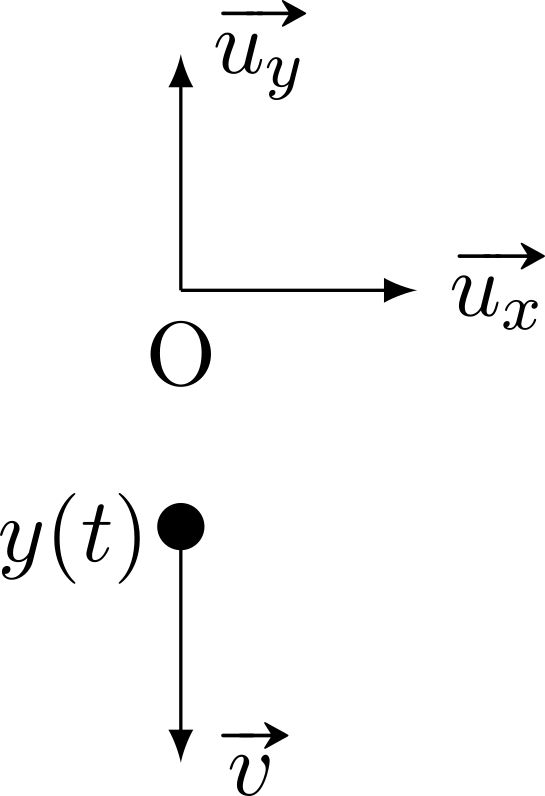
\includegraphics[width=\linewidth]{nov_init}
			\captionsetup{justification=centering}
			\captionof{figure}{}
		\end{center}
	\end{isd}
	\begin{isd}
		\begin{center}
			\sswitch{%
				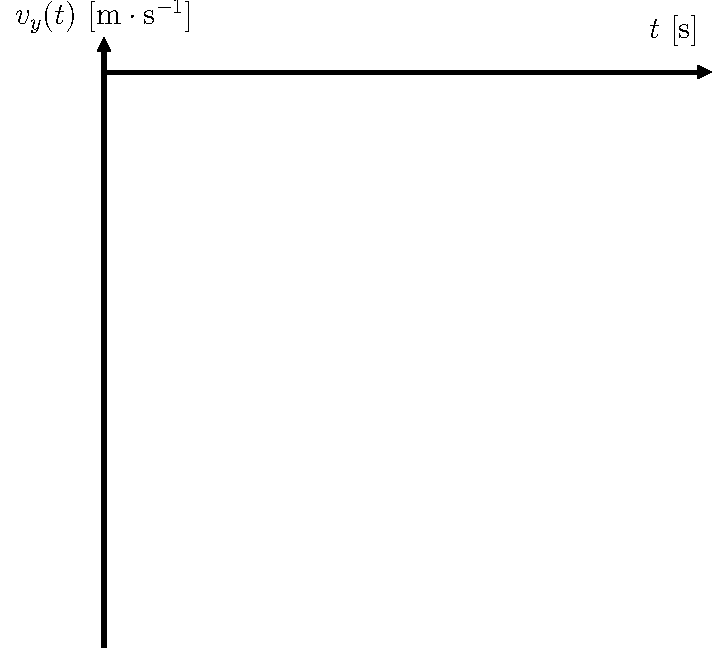
\includegraphics[width=.8\linewidth]{nov_vy_stud}
			}{%
				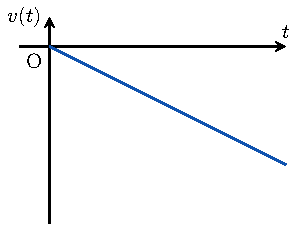
\includegraphics[width=.8\linewidth]{nov_vy_prof}
			}%
			\captionof{figure}{Évolution de $v(t)$.}
		\end{center}
		\tcblower
		\begin{center}
			\sswitch{%
				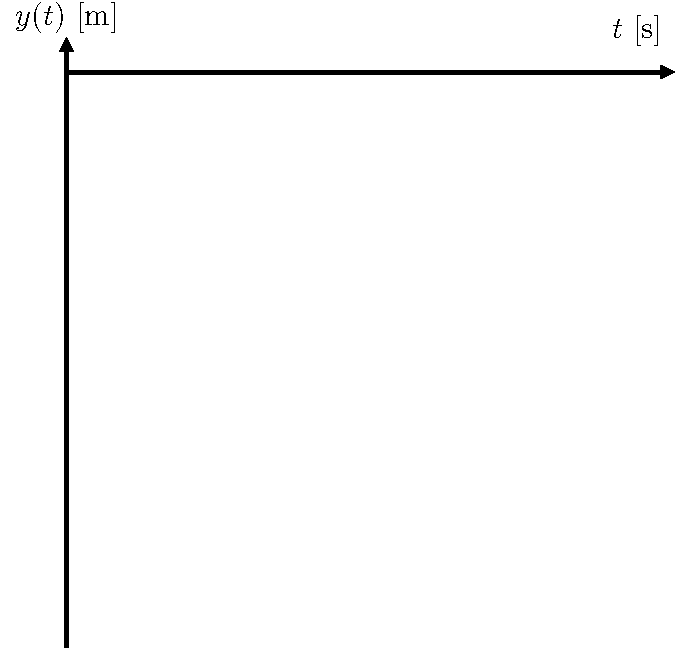
\includegraphics[width=.8\linewidth]{nov_y_stud}
			}{%
				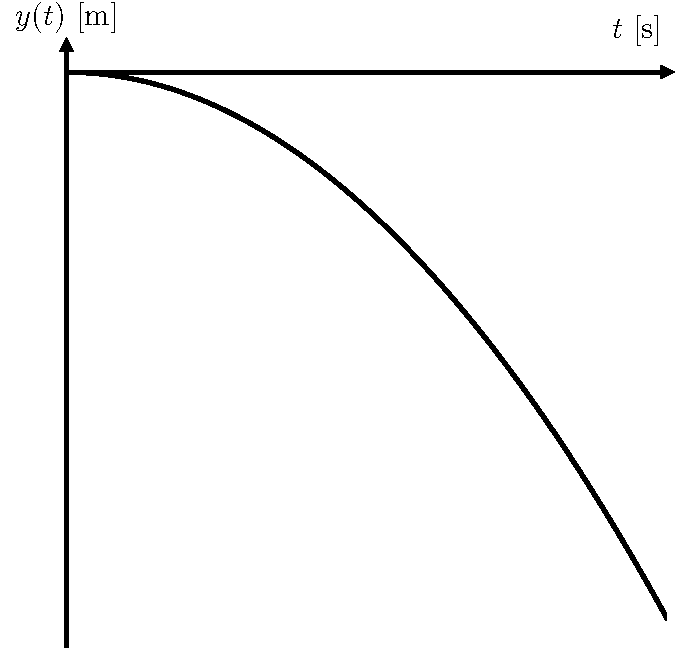
\includegraphics[width=.8\linewidth]{nov_y_prof}
			}%
			\captionof{figure}{Évolution de $y(t)$.}
		\end{center}
	\end{isd}
  \vspace{-25pt}
\end{tcb*}

\subsection{Mouvement courbe uniformément accéléré}
\begin{tcb*}(appl)<lftt>{Mvt. courbe uniformé\mnt\ accéléré}
	Soit $\af(t) = -g\uy$ avec $\vf(0) = v_0\ux$ et $\OM(0) = \of$.
	\begin{enumerate}[label=\sqenumi]
		\item Déterminer les équations horaires.
		\item Déterminer l'équation de la trajectoire.
	\end{enumerate}
	\tcblower
		\begin{enumerate}[label=\sqenumi]
			\item
        \psw{%
          On intègre~:
            \begin{gather*}
              \vf(t) = -gt\uy + \vf(0) = -gt\uy + v_0\ux \Ra
              \OM(t) = -\frac{1}{2}gt^2\uy + v_0t \ux
              \\\beforetext{Soit}
              \boxed{%
                x(t) = v_0t \quad ; \quad
                y(t) = -\frac{1}{2}gt^2
                \quad ; \quad z(t) = 0
              }
            \end{gather*}
        }%
        \vspace{-15pt}
			      \begin{isd}
				      \begin{center}
					      \sswitch{%
						      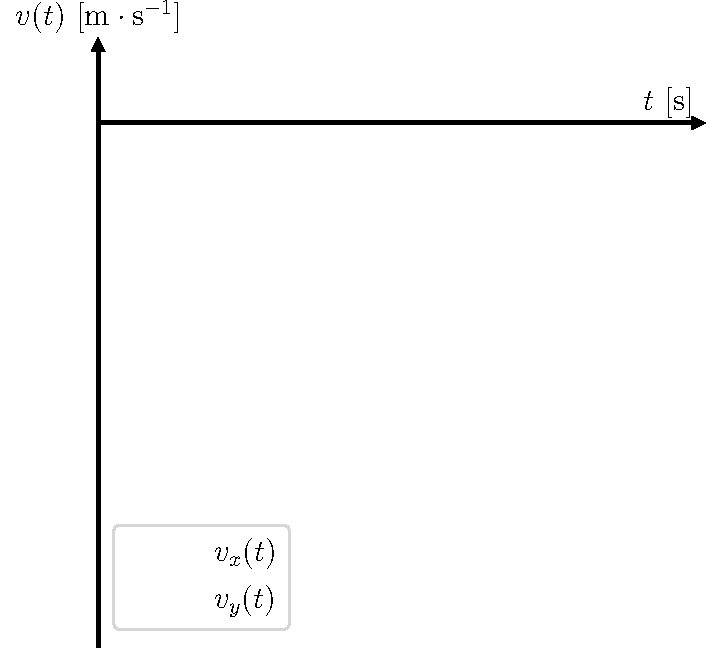
\includegraphics[width=\linewidth]{vo_vv_stud}
					      }{%
						      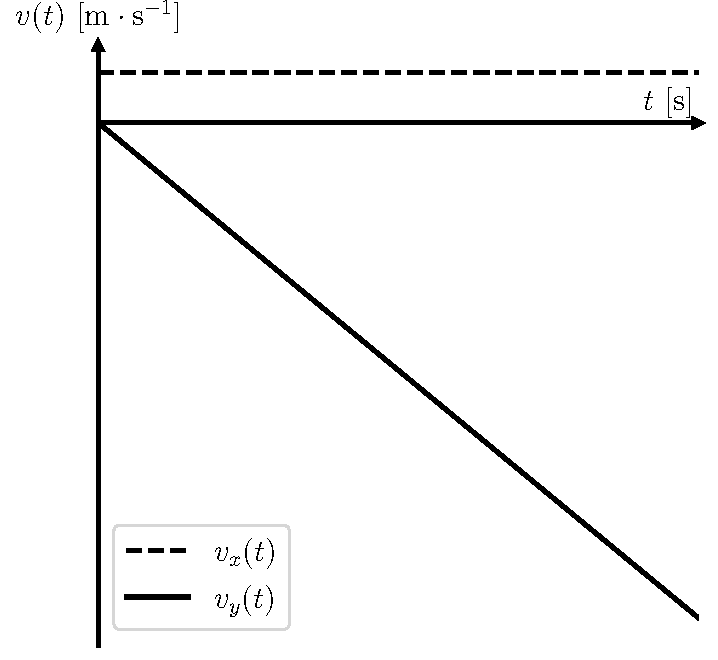
\includegraphics[width=\linewidth]{vo_vv_prof}
					      }%
					      \captionof{figure}{Composantes de la vitesse.}
				      \end{center}
				      \tcblower
				      \begin{center}
					      \sswitch{%
						      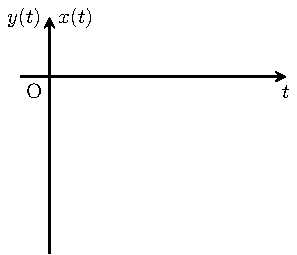
\includegraphics[width=\linewidth]{vo_xx_stud}
					      }{%
						      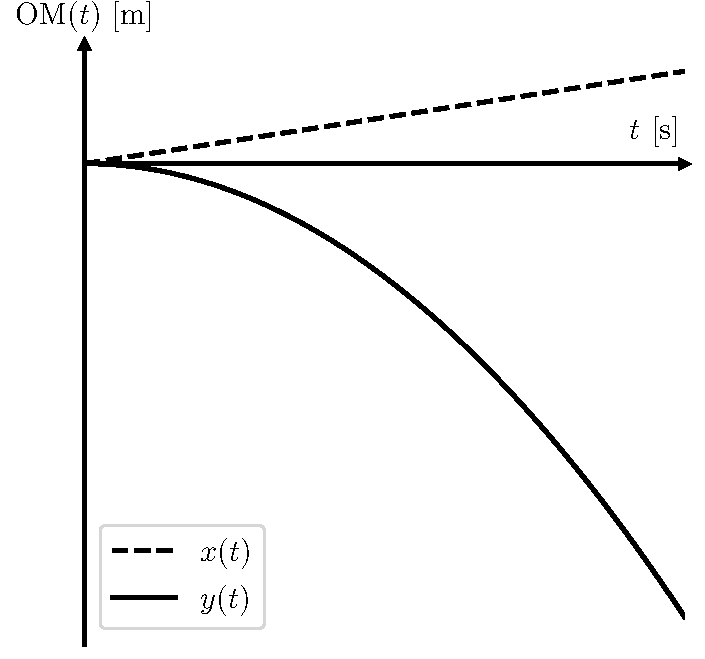
\includegraphics[width=\linewidth]{vo_xx_prof}
					      }%
					      \captionof{figure}{Composantes de la position.}
				      \end{center}
			      \end{isd}
			\item ~
			      \vspace{-15pt}
			      \smallbreak
            \begin{isd}[interior hidden]
              \psw{%
                Pour obtenir la trajectoire, on veut déterminer la courbe $y(x)$
                décrite dans le plan $xy$. Pour cela, exprimons $t$ en fonction de
                $x$ et remplaçons $t$ dans l'expression de $y$~:
                \begin{gather*}
                  t = \frac{x}{v_0}\\
                  \Rightarrow
                  y(x) = - \frac{1}{2}g \left( \frac{x}{v_0} \right)^2
                  \Leftrightarrow
                  \boxed{y(x) = - \frac{g}{2v_0{}^2}x^2}
                \end{gather*}
                La trajectoire obtenue est alors une parabole.
              }%
              \vspace{-15pt}
				      \tcblower
				      \begin{center}
                \sswitch{%
                  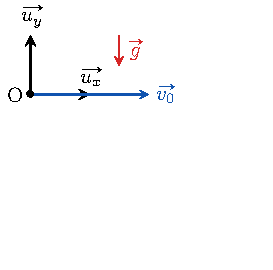
\includegraphics[width=\linewidth]{vo_traj_stud}
                }{%
					        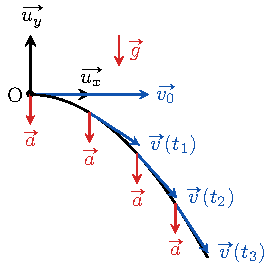
\includegraphics[width=\linewidth]{vo_traj_prof}
                }%
                \vspace{-15pt}
					      \captionof{figure}{Trajectoire parabolique.}
				      \end{center}
			      \end{isd}
		\end{enumerate}
\end{tcb*}

\end{document}
